\documentclass[a4paper,11pt]{article}

\usepackage[dutch]{babel}
\usepackage[utf8]{inputenc}
\usepackage{a4wide,graphicx}
\usepackage{eurosym}
\usepackage{listings}
\usepackage{color}
\usepackage{hyperref}
\usepackage{comment}
\usepackage{float}

\newcommand{\code}[1]{\texttt{#1}}

\begin{document}

\title{SimLogic manual}
\date{}

\maketitle

\emph{This file is licensed under the Apache 2 open source license, see bottom of this document.}

\section{What is SimLogic}

SimLogic is a bare bones logical circuit simulator for educational purposes.
While a great number of sophisticated logic circuit simulators exist,
this one is so simple, that anyone mastering C++ can understand it's sourcecode.

Although the filenames end on \emph{.cpp}, writing simulations requires only \emph{C} knowledge.
However if you want to add special purpose console I/O,
stripped down versions of the C++ streams \emph{cin} and \emph{cout} are available.

It can run on a PC or on an Arduino single board embedded computer.
First \emph{create} circuit elements and then \emph{connect} them, as in the following code:

\begin{lstlisting}[caption={Simulation of a Nand circuit, in the project nand\_example}, numbers=left]
#include "simlogic.h"

int main () {    
    create (Input, inputA);
    create (Input, inputB);
    create (And, anAnd);
    create (Not, aNot);

    connect (inputA, anAnd.inA);
    connect (inputB, anAnd.inB);
    connect (anAnd, aNot.in);

    while (true) {
        evaluate ();
    }
    
    return 0;
}
\end{lstlisting}

The code above will run on a PC under Windows, Linux and OsX, using console I/O.

To make your code run on an Arduino processor board, add I/O blocks as shown below.
Note that, due to the use of \verb!#ifdef!, the code will still run on a PC as well.

\begin{lstlisting}[caption={Nand circuit with Arduino I/O added}, numbers=left]
#include "simlogic.h"

int main () {    
    create (Input, inputA);
    create (Input, inputB);
    create (And, anAnd);
    create (Not, aNot);

    connect (inputA, anAnd.inA);
    connect (inputB, anAnd.inB);
    connect (anAnd, aNot.in);

#ifdef arduino
    pinMode (2, INPUT_PULLUP); pinMode (3, INPUT_PULLUP);
    pinMode (4, OUTPUT); pinMode (5, OUTPUT); pinMode (6, OUTPUT); pinMode (7, OUTPUT);
#endif

    while (true) {
    
#ifdef arduino
        inputA.value = 1 - digitalRead (2); // Inverted because
        inputB.value = 1 - digitalRead (3); // of pull-up resistors
#endif

        evaluate ();
        
#ifdef arduino
        digitalWrite (4, inputA.value);
        digitalWrite (5, inputB.value);
        digitalWrite (6, anAnd.value);
        digitalWrite (7, aNot.value);
#endif 
       
    }    
    return 0;
}
\end{lstlisting}

\section{How it works}

Each SimLogic program is defined in a file called \emph{simulation.cpp}. Note that this one file is the only ``valuable'' user made file in a project. All the rest is boilerplate code, identical for each project. If you want to make a new project \emph{my\_project}, just copy all files from folder \emph{nand\_example} to a new folder \emph{my\_project}. Rename the \emph{.ino} file from \emph{nand\_example.ino} to \emph{my\_project.ino}.
Then edit the \emph{file simulation.cpp} to your liking and compile into an executable using any C++ compiler. The script \emph{compile.bat} requires \emph{gcc} being installed on Windows.

A simulation can run in three ways, depending on macro defintions in \emph{simulation.h}, namely:

\begin{enumerate}
\item{Console I/O on a PC using a command prompt: symbol \emph{console} defined in \emph{simulation.h}, compilation with \emph{compile.bat} on PC}
\item{Console I/O on an Arduino using its IDE's serial monitor: symbol \emph{console} defined, compilation in Arduino IDE. In this case hardware outputs, e.g. LEDs will also work. On the serial monitor, set \emph{Autocroll} on, set the line terminator to \emph{Newline} and set the speed to \emph{9600 baud}. Input happens in one-line entry field at the top of the serial monitor window and is echoed together with output to the multinline text view field at the bottom.}
\item{Hardware I/O on an Arduino, using e.g. buttons and LED's: symbol \emph{console} not defined, compilation in Arduino IDE.}
\end{enumerate}

N.B. A SimLogic program behaves like a PLC (Programmable Logic Controller) rather than a hardwired circuit. This means that its circuit elements are always evaluated in creation order, exactly once for each evaluation cycle (sweep, in PLC terminology). This guarantees that the behaviour is always the same and so called \emph{race conditions} are avoided. It also means that \emph{the creation order of your circuit elements should run from cause to effect}. Pay attention to this, especially if your program behaves differently from what you expect.

\section{Hardware}

When running on an Arduino, connecting buttons and LEDs to the logic circuits provides a visual cue to what's going on.
The hardware for a full adder e.g. looks as follows:

\begin{figure}[H]
\centering
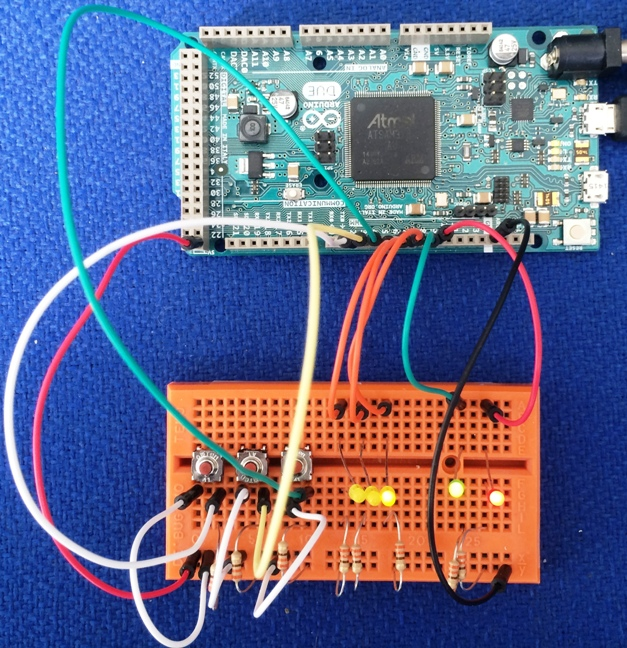
\includegraphics[width=0.7\textwidth]{full_adder.jpg}
\caption{Hardware for the full adder}
\end{figure}

The above circuit uses external resistors to pull the inputs down to ground level (- of the powersupply) when the switches are open.
In that case the I/O mode of the inputs is specified in the code as INPUT.
As can be seen in the example, INPUT\_PULLUP rather than INPUT is used.
This means that the inputs are pulled up to the + level of the power supply when the switches are open.
In that case the external pulldown resistors can be left out.
To prevent the signal from being inverted, the break contact of the switches has te be used.

To gain better insight into the behaviour of the subcircuits and in the way they cooperate to produce the desired output,
the LED's can best be placed into a circuit diagram of the logic that is simulated, like shown below:

\begin{figure}[H]
\centering
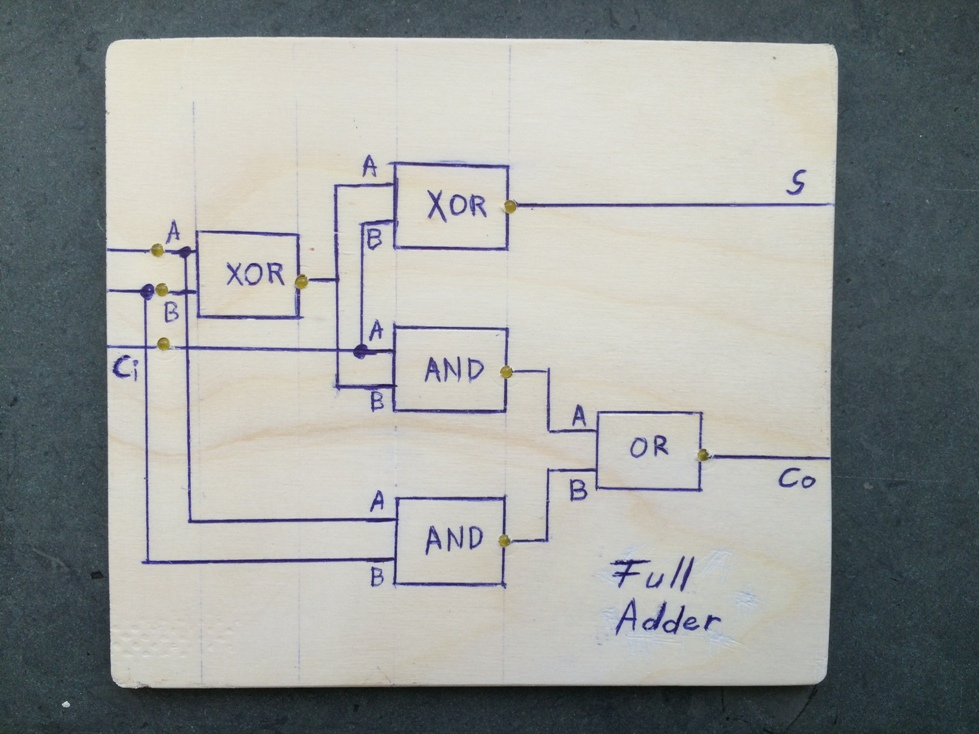
\includegraphics[, width=0.7\textwidth]{full_adder_diagram.jpg}
\caption{Circuit diagram with LED's for the full adder}
\end{figure}
    
\section{Elementary building blocks}

The available circuit element types with their input connectors, used in the \emph{connect} statement, are:

\begin{itemize}
\item{False}
\item{True}
\item{Input: in}
\item{And: inA, inB}
\item{Or: inA, inB}
\item{Xor: inA, inB}
\item{Not: in}
\item{Oneshot: in}
\item{Latch: set, reset}
\end{itemize}
    
\section{Stream I/O}

The simulator has its own bare bones I/O that requires no programming,
it's just there when you use the console.

If you'd like to be fancy and are familiar with C++ you can use \emph{cin} and \emph{cout},
which, on an Arduino, are both of type \emph{SerialStream}:

\begin{lstlisting}
struct SerialStream {
    SerialStream &operator<< (const char * const data);
    SerialStream &operator<< (bool data);
    SerialStream &operator<< (int data);
    SerialStream &operator>> (char * const data);
};
\end{lstlisting}
    
Example of writing something to the console:

\begin{lstlisting}
    cout << "There are " << 2 << " boolean values, namely " << true << " and " << false << endl;
\end{lstlisting}
    
Example of reading a zero terminated string from the console:

\begin{lstlisting}
    cin >> answer;
\end{lstlisting}
    
Note that type SerialStream can be extended by inheritance.
    
\section{Assorted facts and tips}

\begin{itemize}
\item{The project \emph{nand\_example} has been precompiled for Windows with g++ using the \emph{compile.bat} script and will use console I/O.}
\item{Simulations should also compile on Linux and OS X, using appropriate C++ compilers and shell scripts or make files.}
\item{When running in a console window, terminate a simulation simply by CTRL + C.}
\item{There's no error protection, so after an erroneous input it's best to restart the simulation.}
\item{While simulations may use C'ish idiom, still the \emph{.cpp} extension is mandatory.}
\item{Feel free to use C++ rather than C if you're already familiar with the benefits of Object Oriented Programming.}
\item{To instrument your simulation for use with Arduino hardware I/O, add I/O facilities as shown in the \emph{nand\_example}}
\item{To run on an Arduino, go to the directory that holds your project, edit \emph{simulation.h} according to wether or not console I/O is desired, and then use [Sketch][Upload].}
\item{In general the ``everything in one directory'' approach of the Arduino IDE is followed, to keep things simple.}
\end{itemize}

\section{Legal notices}

Copyright 2017 Jacques de Hooge, GEATEC engineering, www.geatec.com

Licensed under the Apache License, Version 2.0 (the ``License'');
you may not use this file except in compliance with the License.
You may obtain a copy of the License at

\url{http://www.apache.org/licenses/LICENSE-2.0}

Unless required by applicable law or agreed to in writing, software
distributed under the License is distributed on an ``AS IS'' BASIS,
WITHOUT WARRANTIES OR CONDITIONS OF ANY KIND, either express or implied.
See the License for the specific language governing permissions and
limitations under the License.

\end{document}

